\documentclass[a4paper,12pt]{jsarticle}

%% パッケージ
\usepackage{enumerate}
\usepackage{ascmac}
\usepackage{amsthm}
\usepackage{enumitem}
\usepackage{amsmath}
\usepackage{amssymb}
\usepackage{amsfonts}
\usepackage{url}
\usepackage[dvipdfmx]{graphicx} 
\usepackage{here}
\usepackage{bm}

%% ここから本文
\begin{document}
扱う反応
\begin{equation*}
\text{Jd}~(\text{NaAlSi}_2\text{O}_6) \to \text{Ab}~(\text{NaAlSi}_3\text{O}_8) + \text{Ne}~(\text{NaAlSiO}_4)
\end{equation*}
系全体のギブスエネルギー変化として, 
\begin{equation*}
(-\Delta G) = (-\Delta G)_{\text{rf}} + (-\Delta G)_{\text{ext}}.
\end{equation*}
各成分について, 
\begin{equation*}
 \bm{n_{\text{Jd}}} = v_{\text{Ab}}\bm{n_{\text{Ab}}} + v_{\text{Ne}}\bm{n_{\text{Ne}}}
\end{equation*}
ここで, 
\begin{equation*}
 \bm{n_{\text{Jd}}} = \begin{pmatrix}
		       n_{\text{Na}}^{\text{Jd}}\\ n_{\text{Al}}^{\text{Jd}}\\ n_{\text{Si}}^{\text{Jd}}
		      \end{pmatrix}, 
 \bm{n_{\text{Ab}}} = \begin{pmatrix}
		       n_{\text{Na}}^{\text{Ab}}\\ n_{\text{Al}}^{\text{Ab}}\\ n_{\text{Si}}^{\text{Ab}}
		      \end{pmatrix}, 
 \bm{n_{\text{Ne}}} = \begin{pmatrix}
		       n_{\text{Na}}^{\text{Ne}}\\ n_{\text{Al}}^{\text{Ne}}\\ n_{\text{Si}}^{\text{Ne}}
		      \end{pmatrix}
\end{equation*}
moral propotionを次のように定義する. 
\begin{equation*}
 m_{\text{Ab}} = \dfrac{v_{\text{Ab}} \Omega_{\text{Ab}}}{v_{\text{Ab}} \Omega_{\text{Ab}} + v_{\text{Ne}} \Omega_{\text{Ne}}},\ m_{\text{Ne}} = 1 - m_{\text{Ab}} = \dfrac{v_{\text{Ne}} \Omega_{\text{Ne}}}{v_{\text{Ab}} \Omega_{\text{Ab}} + v_{\text{Ne}} \Omega_{\text{Ne}}}
\end{equation*}

reaction frontのJd接触における成長速度$v$と, Sym接触における成長速度$u$について, 体積変化反応なので, $u \neq v$. 
体積因子$f_{\Omega}$について,  
\begin{equation*}
 v =u f_{\Omega},\ f_{\Omega} = \dfrac{v_{\text{Ab}} \Omega_{\text{Ab}} + v_{\text{Ne}} \Omega_{\text{Ne}}}{\Omega_{\text{Jd}}}.
\end{equation*}

また反応のギブスエネルギー$G_{\text{re}}$について, 
\begin{equation*}
\Delta G_{\text{re}}  = \Delta_r \overline{g} + \dfrac{2}{\lambda} f_{\Omega} \sigma =\dfrac{\Delta g}{\Omega_{\text{Jd}}} + \dfrac{2}{\lambda}f_{\Omega} \sigma
\end{equation*}
{\Large \textbf{Thermodynamic model for eutectoidal reactions}}

幅$\delta$, フラックス$J_i$, 成長速度$u$, 実効的濃度差$S_i$として,
\begin{align*}
 \delta \dfrac{d J_i}{dy} &= u S_i^{\text{Ne}}\ \left(0 \le y \le \dfrac{\lambda}{2}m_{\text{Ne}}\right)\\
\delta \dfrac{d J_i}{dy} &= u S_i^{\text{Ab}}\ \left(\dfrac{\lambda}{2} m_{\text{Ne}} \le y \le \dfrac{\lambda}{2}\right)
\end{align*}
ここで
\begin{equation*}
 S_i^{\text{Ab}} = \dfrac{n_i^{\text{Jd}}}{\Omega_{\text{Jd}}} - f_{\Omega} \dfrac{n_i^{\text{Ab}}}{\Omega_{\text{Ab}}},\  S_i^{\text{Ne}} = \dfrac{n_i^{\text{Jd}}}{\Omega_{\text{Jd}}} - f_{\Omega} \dfrac{n_i^{\text{Ne}}}{\Omega_{\text{Ne}}}
\end{equation*}
エネルギー散逸を$Q_{\text{diff}}$とすると, 
\begin{equation*}
 Q_{\text{diff}} = \int_V \sum_i J_i X_i dV
\end{equation*}
\begin{figure}[htbp]
 \centering
 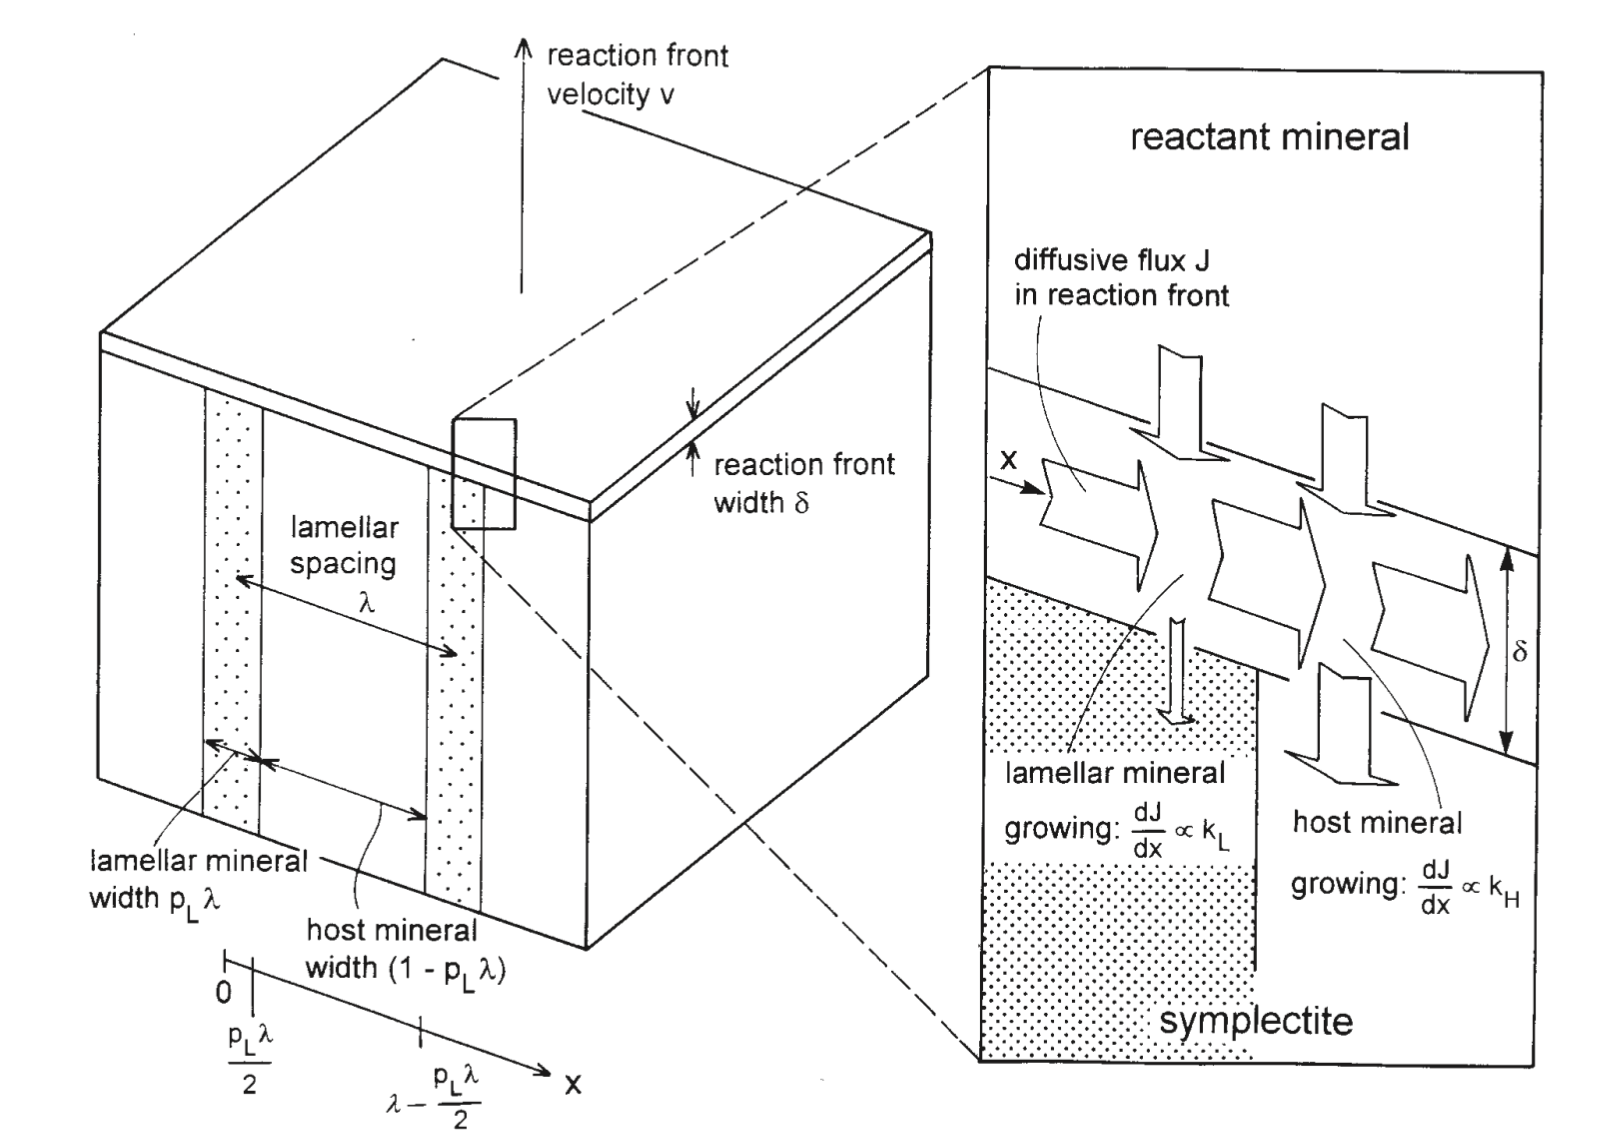
\includegraphics[width=0.9\linewidth]{ashworth1.png}
\caption{lamellar mineral~($=\alpha$)をNe, host~($=\beta$)をAbとした}
\end{figure}
ここで$\displaystyle J_{i} = \sum_{j}L_{i j} \dfrac{d \mu_j}{dx} \simeq  L_{ii}\dfrac{d\mu_i}{dx} \therefore X_i = \dfrac{J_i}{L_{ii}}$.
また, $J_i$に関して積分をして, 
\begin{equation*}
 J_i  = \begin{cases}
	 \dfrac{u}{\delta} S_i^{\text{Ne}} y\ \left(0\le y \le \dfrac{\lambda}{2}m_{\text{Ne}}\right)\\
	 \dfrac{u}{\delta} S_i^{\text{Ab}} \left(y-\dfrac{\lambda}{2}\right) \ \left(\dfrac{\lambda}{2}m_{\text{Ne}} \le y \le \dfrac{\lambda}{2} \right)
	\end{cases}
\end{equation*}
ラメラ1ユニットあたりのエネルギー散逸を求めると, 
\begin{align*}
 Q_{\text{diff}} &= \int_0^\delta \int_0^{\frac{\lambda}{2}} \sum_i \dfrac{J_i^2}{L_{ii}}dx dy = \sum_i\int_0^\delta\left(\int_0^{\frac{\lambda}{2}m_{\text{Ne}}} \dfrac{u^2 (S_i^{\text{Ne}})^2}{\delta^2L_{ii}} y^2dy + \int_{\frac{\lambda}{2}m_{\text{Ne}}}^{\frac{\lambda}{2}} \dfrac{u^2 (S_i^{\text{Ab}})^2}{\delta^2L_{ii}}\left(y-\dfrac{\lambda}{2}\right)^2 dy\right)\\
&= \sum_i \dfrac{u^2}{3\delta L_{ii}}\left((S_i^{\text{Ne}})^2\left(\dfrac{\lambda}{2}m_{\text{Ne}}\right)^3-(S_i^{\text{Ab}})^2\left(\dfrac{\lambda}{2}m_{\text{Ne}}-\dfrac{\lambda}{2}\right)^3\right) \\
&= \sum_i \dfrac{u^2\lambda^3}{24\delta L_{ii}}\left((S_i^{\text{Ne}})^2m_{\text{Ne}}^3 + (S_i^{\text{Ab}})^2(1-m_{\text{Ne}})^3\right)
\end{align*}
つまり界面1 $\text{m}^2$あたりのエネルギー散逸は, 
\begin{align*}
Q_{\text{diff}} &= \sum_i \dfrac{u^2\lambda^3}{24\delta L_{ii}}\left((S_i^{\text{Ne}})^2m_{\text{Ne}}^3 + (S_i^{\text{Ab}})^2(1-m_{\text{Ne}})^3\right)/(\lambda/2) \\
&= \sum_i \dfrac{u^2\lambda^2}{12 \delta L_{ii}}((S_i^{\text{Ne}})^2m_{\text{Ne}}^3+(S_i^{\text{Ab}})^2(1-m_{\text{Ne}})^3)\\
&= u^2 \dfrac{\lambda^2}{\delta}\sum_i \dfrac{(S_i^{\text{Ne}})^2m_{\text{Ne}}^3+(S_i^{\text{Ab}})^2(1-m_{\text{Ne}})^3}{12}\\
&= u^2 \dfrac{\lambda^2}{\delta M_{\text{diff}}}.
\end{align*}
ここで, 系のギブスエネルギーの変化を追うと, 外的な物質供給による変化$(-\Delta G)_{\text{ext}}$と, reaction frontにおけるギブスエネルギー変化$(-\Delta G)_{\text{rf}}$に分けられる. $(-\Delta G)_{\text{ext}}$は分解元の鉱物の反応速度$v$に比例すると考えられるので, 
\begin{equation*}
 (-\Delta G)_{\text{ext}} = sv.
\end{equation*}
また, $(-\Delta G)_{\text{rf}}$は, reaction front内の拡散による変化$(-\Delta G)_{\text{diff}}$


\end{document}